% Introduction
\newpage
\section{Introduction}
\subsection{Background}
Since tennis became popular worldwide, coaches and players have been eager to improve their game by gathering information during the match. Like any other game, the situation in a tennis match is constantly changing. The vast swings, sometimes for many points or even games, that occur in favor of a player who seemed to have the advantage are often attributed to “momentum.” These swings and changes make the game more intense and exciting.

In this thesis, we aim to develop a way to visualize the ups and downs of the game so that coaches and players can analyze the game more scientifically and rationally.

\subsection{Restatement of Problems}
After analyzing the problem's background and question requirements, we have summarized the problem into the following sections:

\begin{itemize}
    \item Capturing the game process through modeling and applying it to the actual game.
    \item Determine if momentum actually affects the course of the game.
    \item Develop a model and analyze whether indicators show the advantage shifts from one athlete to another during a match.
    \item Evaluate our models and make our work visualizable.
\end{itemize}

\subsection{Our Work}
Our work can be summarized into several parts , shown as Figure \ref{fig:OurWork}:
\begin{figure}[b!]
    \centering
    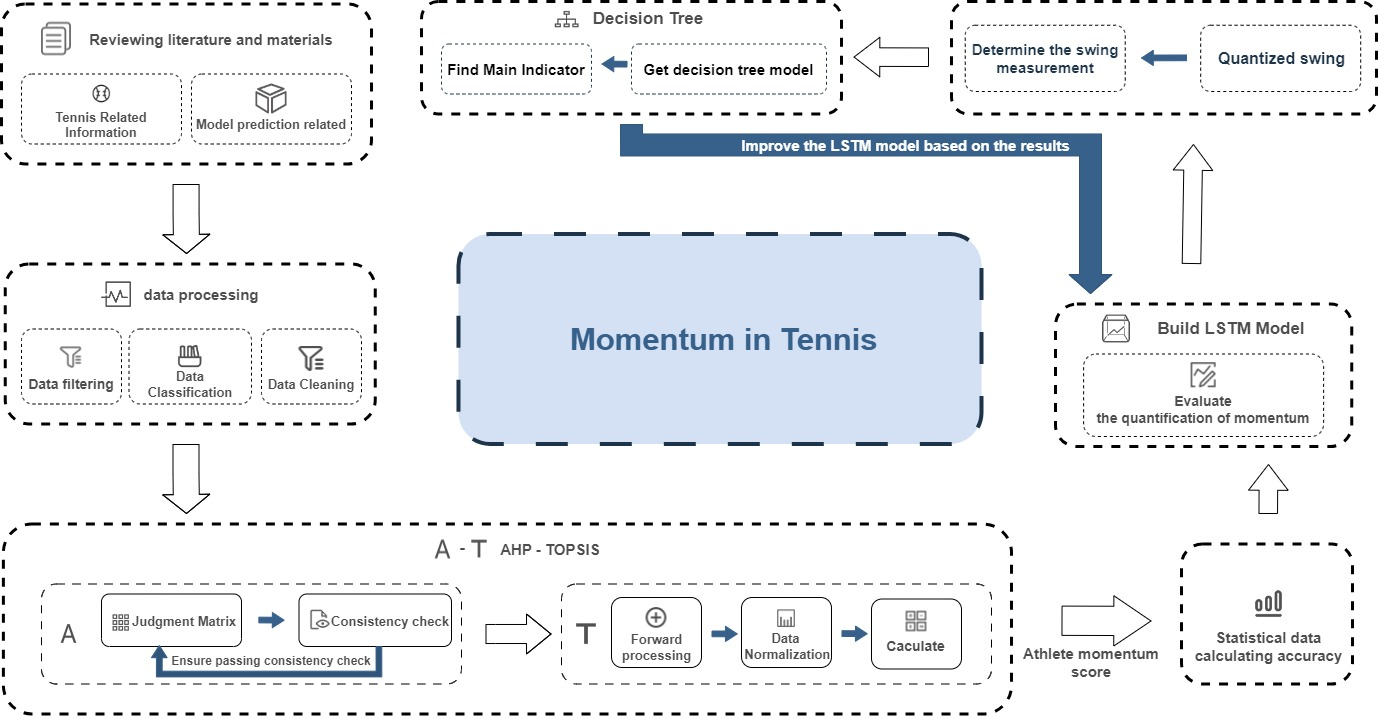
\includegraphics[width=1\linewidth]{figure/OurWork.jpg}
    \caption{\centering Our Work}
    \label{fig:OurWork}
\end{figure}
\begin{itemize}
    \item Search for relevant information on tennis and literature on model prediction
    \item Data processing: filtering, classifying and cleaning data
    \item Determine the weight of factors affecting player momentum in tennis matches through AHP
    \item Accuracy of statistical preliminary data predictions
    \item Create lstm, evaluate the situation of momentum quantification and quantify Swing
    \item Build a decision tree model, find the main indicator, and improve the LSTM model based on it
    \item Get conclusion
\end{itemize}
